\section{Vanishing Point and Lines Detection Program}
\label{sec:program}

This program is designed to detect vanishing points and vanishing lines within images.
It is implemented in Python and is organized into multiple scripts, each dedicated to a specific aspect of the task.

\subsection{Reasoning behind the program}
\label{subsec:reasoning}

The development of the Vanishing Point and Lines Detection Program is driven by the compelling need to extract valuable geometric insights from images,
particularly the identification of converging parallel lines towards a vanishing point.
This information holds substantial significance across various domains, including computer vision, augmented reality, and architectural design.\\
The program is designed to provide a robust and efficient solution for the detection of vanishing points and lines
without the need for manual parameter specification.
The program's functionality can be divided into four main stages:

\begin{itemize}
    \item \textbf{Preprocessing:} This initial step involves transforming the input image into a grayscale format and reducing noise.
          It prepares the image for subsequent analysis by enhancing its clarity and reducing unwanted artifacts.
    \item \textbf{Edge Detection:} Following preprocessing, the program detects edges within the image.
    \item \textbf{Lines Detection:} In this phase, the program identifies and extracts straight line segments from the image.
    \item \textbf{Vanishing Point Detection:} The final and most critical stage involves identifying the vanishing point and vanishing lines within the image.
\end{itemize}


\subsubsection*{Edge Detection}
\label{subsubsec:edge-detection}

Edge detection is a fundamental component of the program, aimed at identifying significant transitions in intensity within an image.
These transitions often correspond to object boundaries or structural elements, providing essential cues for further analysis.
To achieve edge detection, the program employs the Canny edge detector, a multi-stage algorithm that consists of several steps:

\begin{itemize}
    \item \textbf{Noise Reduction}
    \item \textbf{Gradient Computation}
    \item \textbf{Non-Maximum Suppression}
    \item \textbf{Hysteresis Thresholding}
\end{itemize}
\noindent
The values of the "low threshold" and "high threshold" parameters for the Canny edge detector are not fixed
but rather computed dynamically based on the image's intensity distribution.
Specifically, the program calculates these thresholds using the median of the image's intensity distribution,
and the thresholds are set to the computed median $\pm 0.22$.
This adaptive approach ensures that edge detection remains effective across a wide range of images, adapting to variations in lighting and content.
\subsubsection*{Lines Detection}
\label{subsubsec:lines-detection}

The lines detection component of the program is responsible for identifying straight line segments within the image.
These lines can represent a variety of linear structures, including architectural elements, road markings, and other prominent linear features.\\
To accomplish this task, the program employs the probabilistic Hough transform, a widely-used technique for line detection in images.
The Hough transform works by mapping image points to a parameter space where lines are represented as points.
However, the Hough transform involves several parameters that require careful tuning to achieve accurate results.\\
Due to the sensitivity of the Hough transform to parameter settings and the potential for returning different lines based on these parameters,
our approach involves running the Hough transform multiple times, each with a different set of parameters.
By varying the parameters and accumulating the resulting lines, we increase the program's ability to capture a wide range of potential vanishing lines
present in the image.\\
To reduce the number of lines, a decision was made to consider only the five longest lines for each combination of parameters.
Additionally, since parallel and vertical lines are unlikely to be vanishing lines, they are removed.

\subsubsection*{Vanishing Point Detection}
\label{subsubsec:vanishing-point-detection}

Before discussing the implementation, it is important to understand the concepts of the vanishing point and vanishing lines. \\
The vanishing point refers to the point where most of the lines in the image converge. Vanishing lines are the lines that intersect at the vanishing point.
Therefore, the challenge of finding the vanishing point can be reduced to identifying the lines that intersect at a common point.\\
To achieve this, the RANSAC algorithm is employed. Since there are often a large number of detected lines,
it is not feasible to consider all of them for efficiency reasons.
Therefore, the algorithm iterates 500 times, randomly selecting two lines in each iteration to calculate their point of intersection.\\
For each intersection point, the algorithm counts the number of lines passing within a distance of 5 pixels from it.
The point with the highest number of lines passing within this 5-pixel distance is considered the vanishing point.
The lines that pass within 5 pixels of this point are identified as the vanishing lines.\\
To make the results more comprensible to the user, the program draws the vanishing point and the 15-longest vanishing lines on the image.
\subsection{How to use from command line}
The program accepts the following command line arguments:
\begin{itemize}
    \item \texttt{-h} or \texttt{--help}: show the help message and exit.
    \item \texttt{-p} or \texttt{--path}: Specify the path to the input image or a folder containing images for batch processing.
    \item \texttt{-t} or \texttt{--tuning\_method}: Choose the tuning method, either 'Auto' or 'Manual.'
    \item \texttt{-l} or \texttt{--lowThreshold}: Set the low threshold for the Canny edge detector (only for 'Manual' tuning).
    \item \texttt{-r} or \texttt{--highThreshold}: Set the high threshold for the Canny edge detector (only for 'Manual' tuning).
    \item \texttt{-a} or \texttt{--theta}: Set the theta value for the Hough transform (only for 'Manual' tuning).
    \item \texttt{-d} or \texttt{--threshold}: Set the threshold value for the Hough transform (only for 'Manual' tuning).
    \item \texttt{-m} or \texttt{--minLineLength}: Set the minimum line length for the Hough transform (only for 'Manual' tuning).
    \item \texttt{-g} or \texttt{--maxLineGap}: Set the maximum line gap for the Hough transform (only for 'Manual' tuning).
    \item \texttt{-s} or \texttt{--storingPath}: Specify the path to store the output image + name.
\end{itemize}
\noindent
For ’Auto’ tuning method:
\begin{bashscript}
    python vanishingPointDetection.py -p ../Images/vanishing_points  -t Auto -s ../Images/vanishing_points/results
\end{bashscript}
For ’Manual’ tuning, you can use the following command:
\begin{bashscript}
    python3 vanishingPointDetection.py -p ../Images/vanishing_points  -t Manual -l 30 -r 55 -a 1 -d 100 -m 20 -g 16
\end{bashscript}

\subsection{Examples}

These are some examples of the program's output:

\begin{bashscript}
    python3 vanishingPointDetection.py -p ../Images/vanishing_points/van_points.jpeg -t Auto -s ../Images/examples/van_points.jpeg
\end{bashscript}

\begin{figure}[H]
    \centering
    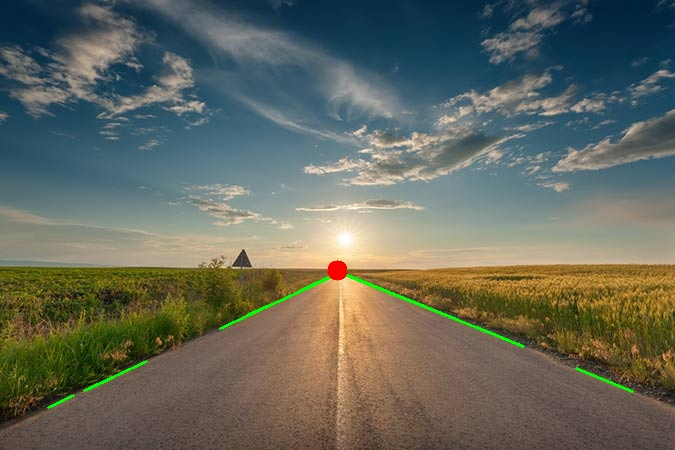
\includegraphics[width=0.4\columnwidth]{../Images/examples/van_points.jpg}
    \caption{Result of the vanishing point detection on the image van\_points.jpg}
    \label{fig-6}
\end{figure}


\begin{bashscript}
    python3 vanishingPointDetection.py -p ../Images/vanishing_points/van_points8.jpeg -t Auto -s ../Images/examples/van_points8.jpeg
\end{bashscript}

\begin{figure}[H]
    \centering
    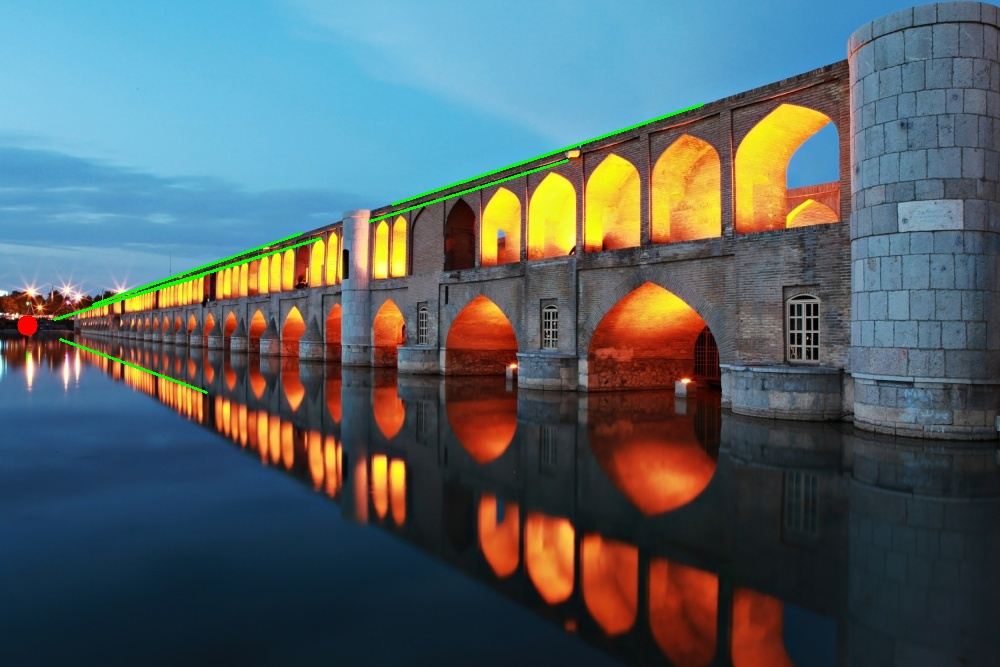
\includegraphics[width=0.4\columnwidth]{../Images/examples/van_points8.jpg}
    \caption{Result of the vanishing point detection on the image van\_points8.jpg}
    \label{fig-7}
\end{figure}


\begin{bashscript}
    python3 vanishingPointDetection.py -p ../Images/vanishing_points/van_points13.jpeg -t Auto -s ../Images/examples/van_points13.jpeg
\end{bashscript}

\begin{figure}[H]
    \centering
    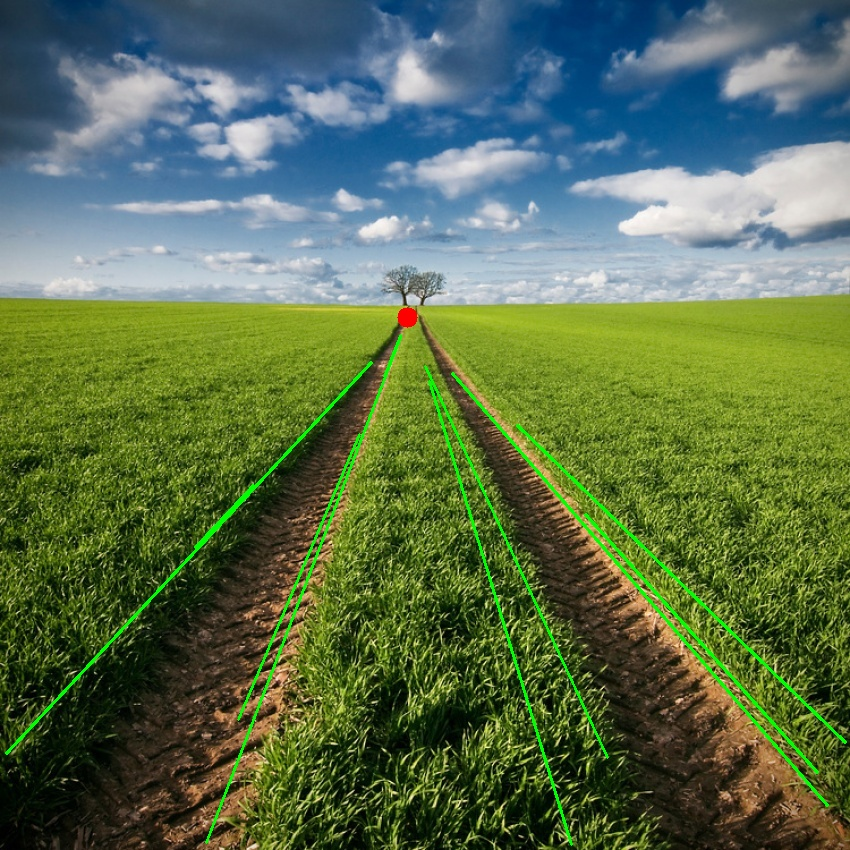
\includegraphics[width=0.4\columnwidth]{../Images/examples/van_points13.jpg}
    \caption{Result of the vanishing point detection on the image van\_points13.jpg}
    \label{fig-8}
\end{figure}

\begin{bashscript}
    python3 vanishingPointDetection.py -p ../Images/vanishing_points/van_points6.jpeg -t Auto -s ../Images/examples/van_points6.jpeg
\end{bashscript}

\begin{figure}[H]
    \centering
    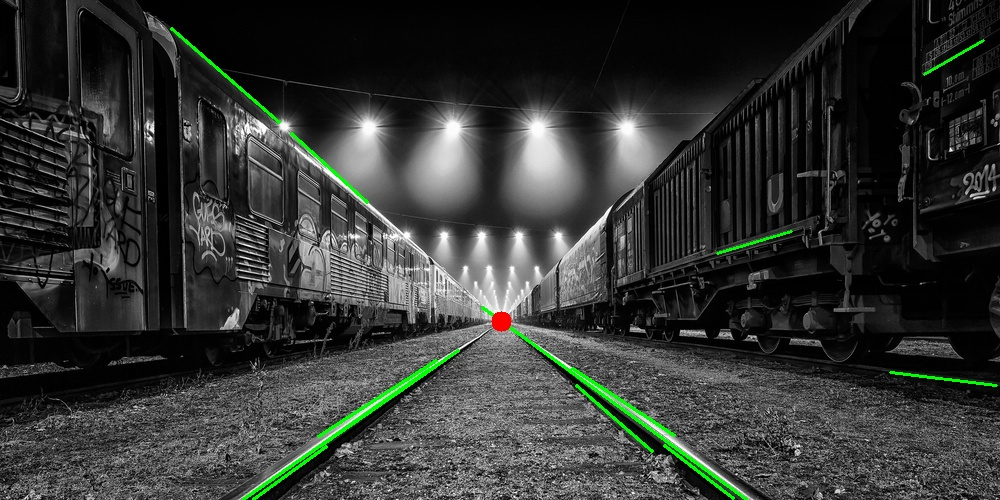
\includegraphics[width=0.4\columnwidth]{../Images/examples/van_points6.jpg}
    \caption{Result of the vanishing point detection on the image van\_points6.jpg}
    \label{fig-9}
\end{figure}